\documentclass[a4paper,11pt]{article}

\usepackage[margin=2.5cm]{geometry}
\usepackage{amsmath,amssymb,amsthm,amsfonts}
\usepackage{enumerate}
\usepackage{mathabx}
\usepackage{braket}
\usepackage[framemethod=tikz]{mdframed}
\usepackage{dsfont}
\usepackage{listings}
\usepackage{color}
\definecolor{dkgreen}{rgb}{0,0.6,0}
\definecolor{gray}{rgb}{0.5,0.5,0.5}
\definecolor{mauve}{rgb}{0.58,0,0.82}
\usepackage{fancyhdr}
\usepackage{graphicx}
\usepackage{epstopdf}
\usepackage{pgfplots}
\usepackage{tikz}
\usepackage{pgfplots}
\usepackage{placeins}
\usepackage{flafter}

\lstset{frame=tb,
	language=C++,
	aboveskip=3mm,
	belowskip=3mm,
	showstringspaces=false,
	columns=flexible,
	basicstyle={\small\ttfamily},
	numbers=none,
	numberstyle=\tiny\color{gray},
	keywordstyle=\color{blue},
	commentstyle=\color{dkgreen},
	stringstyle=\color{mauve},
	breaklines=true,
	breakatwhitespace=true,
	tabsize=3
}

\newtheorem*{remark}{Remark}

\newtheoremstyle{break}
{\topsep}{\topsep}%
{\itshape}{}%
{\bfseries}{}%
{\newline}{}%
\theoremstyle{break}

\newtheoremstyle{break2}
{\topsep}{\topsep}%
{}{}%
{\bfseries}{}%
{\newline}{}%
\theoremstyle{break2}

\theoremstyle{break}
\newtheorem{theorem}{Theorem}[section]
\newtheorem{proposition}[theorem]{Proposition}
\newtheorem{corollary}[theorem]{Corollary}
\newtheorem{lemma}[theorem]{Lemma}

\theoremstyle{break2}
\newtheorem{definition}[theorem]{Definition}
\newtheorem{example}[theorem]{Example}

\newcommand{\R}{\mathbb{R}}
\newcommand{\N}{\mathbb{N}}
\newcommand{\Z}{\mathbb{Z}}
\newcommand{\Q}{\mathbb{Q}}
\newcommand{\C}{\mathbb{C}}
\newcommand{\F}{\mathbb{F}}
\newcommand{\K}{\mathbb{K}}
\newcommand{\lP}{\mathbb{P}}
\newcommand{\lS}{\mathbb{S}}
\newcommand{\cA}{\mathcal{A}}
\newcommand{\cB}{\mathcal{B}}
\newcommand{\cL}{\mathcal{L}}
\newcommand{\cF}{\mathcal{F}}
\newcommand{\cO}{\mathcal{O}}
\newcommand{\cM}{\mathcal{M}}
\newcommand{\cC}{\mathcal{C}}
\newcommand{\cE}{\mathcal{E}}
\newcommand{\cP}{\mathcal{P}}
\newcommand{\s}{\sigma}
\newcommand{\e}{\varepsilon}
\newcommand{\Cyl}{\textnormal{Cyl}}
\newcommand{\de}{\textnormal{ d}}
\newcommand{\I}{\mathds{1}}
\newcommand{\wto}{\rightharpoonup}

\title{C1 - Assignment 4 Report}
\author{Student Number: u1858921}
\date{Submission Deadline: 6pm December 27th, 2018}

\begin{document}
	\maketitle
	\tableofcontents
	
\section{Introduction}
In this report, we discuss and describe a way to numerically solve the heat equation under suitable boundary and initial conditions by first discretising space and then solving the resulting IVP. This method is known as the \emph{method of lines}.
\begin{mdframed}
	The heat equation is given as follows. For $ \kappa \in \R $ (a diffusivity parameter), solve the following equation for $ u : I \times \Omega \to \R $:
	\begin{align*}
	u_t(t,x) &= \kappa u_{xx}(t,x) \quad (t,x) \in I \times \Omega \\
	u(0,x) &= u_0(x) \\
	u(t,x) &= 0 \quad (t,x) \in I \times \partial\Omega,
	\end{align*}
	for the initial condition function $ u_0 : \Omega \to \R $ given.
\end{mdframed} 
\noindent
Throughout this report we shall discuss the theoretical discretisation and the problem set up and then discuss the numerical implementation of the method of lines. We then test the numerical implementation with test values for $ \kappa $ and the spatial and temporal discretisation step size.

\section{Problem}
The aim of this assignment is to solve the following parabolic initial-boundary value problem for $ u(x,t) : \Omega \times I \to \R $ given by
\begin{align}
\begin{cases}
\partial_t u(x,t) = \kappa \partial_x^2 u(x,t) & (x,t) \in \Omega \times I \\
u(x,0) = u_0(x) & x \in \Omega,
\end{cases}
\end{align}
i.e. the \emph{heat equation}, with periodic boundary conditions on $ \Omega = [0,L = 1] $ with $ I = [0, T = 0.1] $, where
\begin{align*}
u_0(x) =
\begin{cases}
0 & \text{if } x \leq \frac{1}{4} \text{ or } x > \frac{3}{4}, \\
1 & \text{otherwise}.
\end{cases}
\end{align*}

\subsection{Method of Lines}
Let $ N_x $ and $ N_t $ denote the number of spatial and temporal discretisation points respectively. Further let $ (x_i)_{i=0}^{N_x + 1} $ be a set of points, that discretise $ \Omega = [0,1] $, such that
\begin{align*}
0 = x_0 < x_1 < \cdots < x_{N_x} < x_{N_x + 1} = 1.
\end{align*}
Denote by $ I_k := [x_{k},x_{k+1}] $ and let $ |I_k| = x_{k+1} - x_{k} := h $ for some $ h \in \R $ (the spatial mesh size) for $ k = 0,\ldots,N_x $. Denote by $ U_i : I \to \R $ the approximation of the exact solution $ u $ at $ x_i $ for $ i = 1,\ldots,N_x $.
\\\\
We begin the method of lines discertisation by first discretising the spatial direction with second order central finite differences to obtain an initial value problem, that is for $ i = 1,\ldots,N_x $
\begin{align*}
\frac{\de U_i}{\de t} &= \kappa \partial^+\partial^- U_i = \kappa\frac{U_{i+1} - 2U_i + U_{i-1}}{h^2}.
\end{align*}
Then if we denote by $ \mathbf{U} = (U_1,\ldots,U_{N_x}) : I^{N_x} \to \R $, then we may rewrite the series of IVPs as follows (taking into account the boundary conditions that we impose) 
\begin{align}\label{Eq:IVP from Method of Lines}
\frac{\de \mathbf{U}}{\de t} = -\frac{\kappa}{h^2}
\begin{pmatrix}
2 & -1 & & & & \\
-1 & 2 & -1 & & & \\
& -1 & 2 & -1 & & \\
& & \ddots & \ddots & \ddots & \\
& & & & & -1 \\
& & & & -1 & 2
\end{pmatrix}
\mathbf{U} =: f(t,\mathbf{U}).
\end{align}
We solve \eqref{Eq:IVP from Method of Lines} using one-step methods, in particular the Runge-Kutta method. Before we describe the Runge-Kutta implementation, we discretise the temporal space. That is, let $ (t_n)_{n = 0}^{N_t + 1} $ denote the discretisation of the temporal space $ I = [0,0.1] $, such that
\begin{align*}
0 = t_0 < t_1 < \cdots < t_{N_t} < t_{N_t + 1} = 0.1.
\end{align*}
Denote by $ J_k := [t_{k},t_{k+1}] $ and let $ |J_k| = t_{k+1} = I_{k} := \tau $, for some $ \tau \in \R $ (the temporal step size) for $ k = 0,\ldots,N_t $. Denote by $ \mathbf{U}^{l} $ the approximation of the exact solution of the IVP $ \mathbf{U} $ at $ t_i $ for $ i = 1,\ldots,N_t $. Additionally denote $ f(t_i,\mathbf{U}^i) = f_i $.
\\\\
Now the $ s $-stage Runge-Kutta method for the IVP \eqref{Eq:IVP from Method of Lines} is of the form
\begin{align*}
\mathbf{U}^{n+1} = \mathbf{U}^{n} + \tau F(t_n, \mathbf{U}^n, f, \tau),
\end{align*}
where the increment function $ F $ is defined as
\begin{align*}
F(t_n, \mathbf{U}^n, f, \tau) &= \sum_{i=1}^{s}b_iK_i \\
K_i &= f\left(t_n + c_i\tau, \mathbf{U}^n + \tau\sum_{j=1}^{s}a_{ij}K_j\right), \quad \text{for } i \in \{1,\ldots,s\},
\end{align*}
and $ A = (a_{ij}) \in \R^{s \times s} $, $ \mathbf{b}, \mathbf{c} \in \R^s $ completely determine the Runge-Kutta method. We shall denote a specific Runge-Kutta method by a \emph{Butcher tableau} of the following form
\begin{align*}
\renewcommand\arraystretch{1.2}
\begin{array}
{c|c}
\mathbf{c} &
A\\
\hline
& \mathbf{b}
\end{array}.
\end{align*}
The Runge-Kutta schemes that will be of interest in this report are the following, given by their Butcher tableau's
\begin{center}
	\begin{minipage}{0.3\linewidth}
		\begin{align*}
		\renewcommand\arraystretch{1.2}
		\textnormal{Forward Euler (FE)} \\
		\begin{array}
		{c|c}
		0 &
		\\
		\hline
		& 1
		\end{array}
		\end{align*}
	\end{minipage}
	\begin{minipage}{0.3\linewidth}
		\begin{align*}
		\renewcommand\arraystretch{1.2}
		\textnormal{Backward Euler (BE)} \\
		\begin{array}
		{c|c}
		1 & 1
		\\
		\hline
		& 1
		\end{array}
		\end{align*}
	\end{minipage}
	\begin{minipage}{0.3\linewidth}
		\begin{align*}
		\renewcommand\arraystretch{1.2}
		\textnormal{3-stage Heun (Heun3)} \\
		\begin{array}
		{c|ccc}
		0 & & \\
		1/3 & 1/3 & \\
		2/3 & 0 & 2/3 \\
		\hline
		& 1/4 & 0 & 3/4
		\end{array}
	\end{align*}
	\end{minipage}
\end{center}

\subsection{Numerical Implementation}
The numerical implementation extends that of the one made in Assignment 3. That is we implement all the Runge-Kutta schemes in a class format, where we define a general class called \texttt{DIRK} (diagonally implicit Runge-Kutta), with general values for $ A $, $ \mathbf{b} $ and $ \mathbf{c} $. A specific scheme is then implemented using a number of derived classes \texttt{FE}, \texttt{BE}, \texttt{Heun3}, which when called will set the required values for $ A $, $ \mathbf{b} $ and $ \mathbf{c} $ in the general \texttt{DIRK} class. We note that when we have an implicit method, such at the backward Euler scheme, \texttt{BE}, then at each stage we have to determine $ K_i $ for a specific $ i \leq s $ by solving the implicit equation
\begin{align*}
K_i = f\left(t_n + \tau c_i, \mathbf{U}^n + \tau\sum_{j=1}^{i-1}a_{ij}K_j + \tau a_{ii}K_i\right),
\end{align*}
which depends on the previous $ K_i $'s and also on itself, and thus cannot be solved stage by stage. At each stage $ i $, we therefore solve for $ K_i $ through other means, in particular the Newton method. Using the Newton method, we solve for the root of the vector valued function $ g $ given by
\begin{align*}
g(K_i) := f\left(t_n + \tau c_i, \mathbf{U}^n + \tau\sum_{j=1}^{i-1}a_{ij}K_j + \tau a_{ii}K_i\right) - K_i,
\end{align*}
where the root $ K_i $ is approximated through the following iteration equation
\begin{align*}
K_i^{k+1} = K_i^{k} - (g(K_{i}^{k}))^{-1}g(K_{i}^{k}),
\end{align*}
up to some threshold ($ K_i^k $ denotes the $ k $th iteration of the approximation of $ K_i $). This described implementation is given below. We note that to perform the inversion $ (g(K_{i}^{k}))^{-1} $, we make use of one of a number of numerical inversion techniques. For this assignment, we shall use the Gauss-Seidel inversion algorithm implemented in Assignment 1.
\begin{lstlisting}
class DIRK
{
public:

	DIRK(int stages)
		: stages_(stages), a_(stages*stages), b_(stages), c_(stages)
		{
			for (int i=0;i<stages_;++i)
				for (int j=0;j<stages_;++j)
					a_[i*stages_+j] = 0.;
					b_[0] = 1.;
					c_[0] = 0.;
		}

	template <class Model>
	Vector evolve(const Vector &y, double t, double h, const Model &model) const // h  = tau here
	{
		Vector ret = y;
		std::vector<Vector> k(stages_, Vector(model.N));
		for (int s=0; s<stages_; ++s )
		{
			Vector temp_sum = y;
			for (int j = 0; j < s; ++j)
			{
				temp_sum += h*a(s,j)*k[j];
			}
			if (a(s,s) != 0)
			{
				int iter = 0;
				double error = (model.f(t + h*c_[s], temp_sum + h*a(s,s)*k[s]) - k[s]).maxNorm();
				SparseMatrix Jac = model.df(t + h*c_[s], temp_sum + h*a(s,s)*k[s]);
				while (iter < 1e6 && std::abs(error) > 1e-6)
				{
					k[s] = Jac.GaussSeidel((-1)*model.f(t + h*c_[s], temp_sum + h*a(s,s)*k[s]),k[s], 1e-6, 1e6) + k[s];
					error = (model.f(t + h*c_[s], temp_sum + h*a(s,s)*k[s]) - k[s]).maxNorm();
					iter++;
				}
				temp_sum += h*a(s,s)*k[s];
			}
			k[s] = model.f(t + c_[s]*h, temp_sum);
			ret += h*b_[s]*k[s];
		}
		return ret;
	}

protected:

	const double a(int i, int j) const { return a_[i*stages_+j]; }
	double& a(int i, int j) { return a_[i*stages_+j]; }

	int stages_;

	std::vector<double> a_,b_,c_;
};
\end{lstlisting}
Within the class, the function \texttt{evolve} solves the IVP for the time step $ t + \tau $ for values $ t $ and $ \tau $ given in the input. To solve the IVP completely over the interval $ [0,T = 0.1] $, we need to perform the evolution through the \texttt{evolve} function with a given time step $ \tau $. We solve over $ [0,T = 0.1] $ by implementing a function called \texttt{solve}, which takes a function$ f $, a scheme and a discretisation time step $ \tau $, and then computes the solution $ y(t) $ at each $ t_i = i\tau $ whilst $ t_i \in [0,T=0.1] $.
\begin{lstlisting}
template <class Model>
Vector solve(const Model &model, const DIRK &scheme, double tau)
{
	Vector y=model.y0();
	double t=0;
	while ( std::abs(model.T()-t)>tau )
	{
		y =  scheme.evolve(y,t,tau,model);
		t += tau;
	}
	std::cout << "Finished time integration at t=" << t << std::endl;
	return y;
}
\end{lstlisting}

\subsection{Step-size Analysis}


\subsection{Plots}

\begin{figure}[h]
	\centering
	\textbf{Forward Euler}\par\medskip
	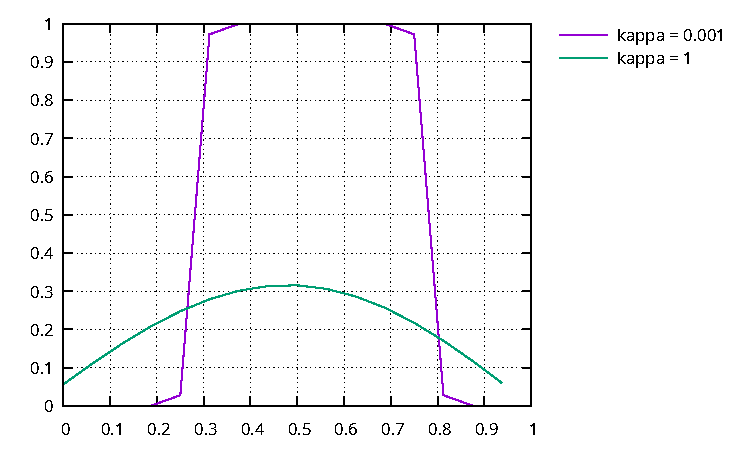
\includegraphics[width=\linewidth]{HE_plot_FE.pdf}
	\caption{$ N_x = 16 $}
\end{figure}

\begin{figure}[h]
	\centering
	\textbf{3 Stage Heun}\par\medskip
	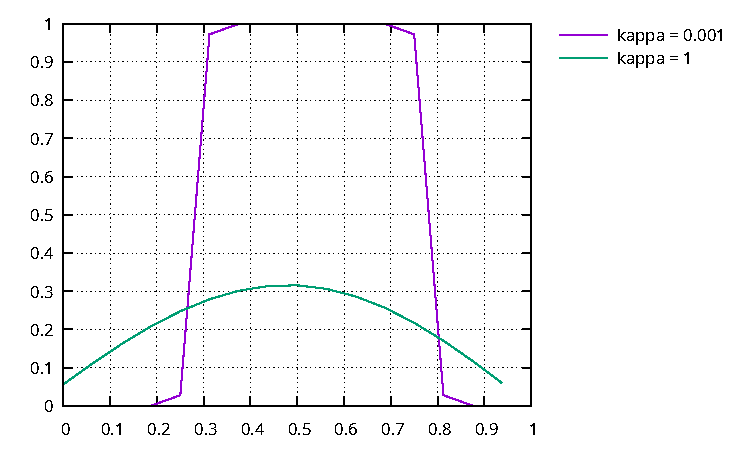
\includegraphics[width=\linewidth]{HE_plot_Heun3.pdf}
	\caption{$ N_x = 16 $}
\end{figure}
\section{Conclusion}



\end{document}
